\documentclass[aspectratio=169]{beamer}

\usepackage{beamerthemesplit}
\usepackage{amsmath}
\usepackage{amsfonts}
\usepackage{amssymb}
\usepackage{cancel}
\usepackage{bussproofs}
\usepackage{graphicx}

% For ⩘ and ⩗ (requires the LuaLaTeX engine)
\usepackage{unicode-math}
\setmathfont{Stix Two Math}

% For highlighting MeTTa code
\usepackage{listings}
\usepackage{color}
\definecolor{mygreen}{rgb}{0,0.6,0}
\definecolor{mygray}{rgb}{0.5,0.5,0.5}
\definecolor{mymauve}{rgb}{0.58,0,0.82}
\lstset{ %
  backgroundcolor=\color{white},   % choose the background color
  basicstyle=\tiny,                % size of fonts used for the code
  breaklines=true,                 % automatic line breaking only at whitespace
  captionpos=b,                    % sets the caption-position to bottom
  commentstyle=\color{mygreen},    % comment style
  escapeinside={\%*}{*)},          % if you want to add LaTeX within your code
  keywordstyle=\color{blue},       % keyword style
  stringstyle=\color{mymauve},     % string literal style
}

% Commands for Atomese code
\newcommand{\SP}{\;\;\;}
\newcommand{\TTrue}{\textit{True}}
\newcommand{\TFalse}{\textit{False}}
\newcommand{\TAtom}{\textit{Atom}}
\newcommand{\TTime}{\textit{Time}}
\newcommand{\TEval}{\textit{Evaluation}}
\newcommand{\TList}{\textit{List}}
\newcommand{\TLamb}{\textit{Lambda}}
\newcommand{\TExec}{\textit{Execution}}
\newcommand{\TAtTime}{\textit{AtTime}}
\newcommand{\TAnd}{\textit{And}}
\newcommand{\TOr}{\textit{Or}}
\newcommand{\TNot}{\textit{Not}}
\newcommand{\TImpl}{\textit{Implication}}
\newcommand{\TPredImpl}{\textit{PredictiveImplication}}
\newcommand{\TSeqAnd}{\textit{SequentialAnd}}
\newcommand{\TSeqOr}{\textit{SequentialOr}}
\newcommand{\TBSeqAnd}{\textit{BackSequentialAnd}}
\newcommand{\TFSeqAnd}{\textit{ForeSequentialAnd}}
\newcommand{\TLag}{\textit{Lag}}
\newcommand{\TLead}{\textit{Lead}}
\newcommand{\TTV}{\textit{TV}}
\newcommand{\TTVo}{\textit{TV}_1}
\newcommand{\TTVi}{\textit{TV}_i}
\newcommand{\TTVn}{\textit{TV}_n}
\newcommand{\TTVPo}{\textit{TV}_1^P}
\newcommand{\TTVQo}{\textit{TV}_1^Q}
\newcommand{\TTVPi}{\textit{TV}_i^P}
\newcommand{\TTVQi}{\textit{TV}_i^Q}
\newcommand{\TTVPn}{\textit{TV}_n^P}
\newcommand{\TTVQn}{\textit{TV}_n^Q}
\newcommand{\TTVP}{\textit{TV}^P}
\newcommand{\TTVQ}{\textit{TV}^Q}
\newcommand{\TTVR}{\textit{TV}^R}
\newcommand{\TTVPQ}{\textit{TV}^{PQ}}
\newcommand{\TTVQR}{\textit{TV}^{QR}}
\newcommand{\TBTV}{\langle \TTV \rangle}
\newcommand{\TBTVPo}{\langle \TTVPo \rangle}
\newcommand{\TBTVQo}{\langle \TTVQo \rangle}
\newcommand{\TBTVPi}{\langle \TTVPi \rangle}
\newcommand{\TBTVQn}{\langle \TTVQn \rangle}
\newcommand{\TBTVPn}{\langle \TTVPn \rangle}
\newcommand{\TBTVQi}{\langle \TTVQi \rangle}
\newcommand{\TBTVP}{\langle \TTVP \rangle}
\newcommand{\TBTVQ}{\langle \TTVQ \rangle}
\newcommand{\TBTVR}{\langle \TTVR \rangle}
\newcommand{\TBTVPQ}{\langle \TTVPQ \rangle}
\newcommand{\TBTVQR}{\langle \TTVQR \rangle}
\newcommand{\Tstrength}{\textit s}
\newcommand{\Tconf}{\textit c}

% Commands for symbolic mathematical notations
\newcommand{\prob}[1]{\mathcal{Pr}\left(#1\right)}
\newcommand{\mean}{\textit{mean}}
\newcommand{\cnt}{\textit{count}}
\newcommand{\poscnt}{\textit{pos\_count}}
\newcommand{\sat}[1]{\mathcal{S}(#1)}
\newcommand{\ltv}[1]{<\!\!#1\!\!>}
\newcommand{\letv}[2]{(#1, #2)}
\newcommand{\limp}{\rightarrow}
\newcommand{\lpreimp}[1]{\leadsto^{#1}}
\newcommand{\lseqor}[1]{\bigslopedvee^{#1}}
\newcommand{\lseqand}[1]{\bigslopedwedge^{#1}}
\newcommand{\lbseqor}[1]{\reflectbox{$\bigslopedvee$}^{#1}}
\newcommand{\lbseqand}[1]{\reflectbox{$\bigslopedwedge$}^{#1}}
\newcommand{\ldo}[1]{\widehat{#1}}
\newcommand{\llag}[2]{\overrightarrow{#1}^{#2}}
\newcommand{\llead}[2]{\overleftarrow{#1}^{#2}}

\makeatletter
\newcommand{\reallytiny}{\@setfontsize{\srcsize}{2pt}{2pt}}
\makeatother

\mode<presentation>
{
  \usetheme{AnnArbor}
  \usecolortheme{crane}
}

\usepackage[english]{babel}
%% \usepackage[latin1]{inputenc}
\usepackage{times}
\usepackage[T1]{fontenc}

\title{Rational OpenCog Controlled Agent}

\author{Nil Geisweiller, Hedra Yusuf}

\institute[SingularityNET OpenCog Foundations]
{
  \begin{center}
    AGI-23\\
    
\includegraphics[scale=0.32]{pictures/snet_oc.png}
  \end{center}
}

\date[AGI-23]

\begin{document}

\section{Introduction}

\begin{frame}
  \maketitle
\end{frame}

% %%%%%%%%%%%%%%%%%%%%%%%%%%%%%%%%%%%%%%%%%%%%%%%%%%%%%%%%%%%%%%%%%%%%%%%%%%%
% %% This presentation is gonna be all about porting PLN to MeTTa.  You    %%
% %% might see that the title has been somewhat simplified, that's because %%
% %% we didn't have enough to really touch on the temporal aspect of PLN.  %%
% %%%%%%%%%%%%%%%%%%%%%%%%%%%%%%%%%%%%%%%%%%%%%%%%%%%%%%%%%%%%%%%%%%%%%%%%%%%

% \section{PLN Recall}

% \begin{frame}[fragile]

% %%%%%%%%%%%%%%%%%%%%%%%%%%%%%%%%%%%%%%%%%%%%%%%%%%%%%%%%%%%%%%%%%%%%%%%%%
% %% So let me start by giving a brief recall of what is PLN, and as I   %%
% %% do so I will also introduce some notations that will be used in the %%
% %% PLN MeTTa port.                                                     %%
% %%%%%%%%%%%%%%%%%%%%%%%%%%%%%%%%%%%%%%%%%%%%%%%%%%%%%%%%%%%%%%%%%%%%%%%%%

% %%%%%%%%%%%%%%%%%%%%%%%%%%%%%%%%%%%%%%%%%%%%%%%%%%%%%%%%%%%%%%%%%%%%%%%
% %% I'm only going to recall the portion of PLN that's relevant here, %%
% %% not the whole logic.                                              %%
% %%%%%%%%%%%%%%%%%%%%%%%%%%%%%%%%%%%%%%%%%%%%%%%%%%%%%%%%%%%%%%%%%%%%%%%

%   \frametitle{PLN Recall}

% % %%%%%%%%%%%%%%%%%%%%%%%%%%%%%%%%
% % %% Given a list of predicates %%
% % %%%%%%%%%%%%%%%%%%%%%%%%%%%%%%%%

% % $P, Q, \hdots: \textit{Atom}^n \rightarrow \{\top, \bot\}$
% % {\tiny \alert{(possibly fuzzy)}}

% % \renewcommand{\arraystretch}{1.5}

% % {\small
% % $$
% % \begin{array}{|c|c|c|}
% %   \hline
% %   \text{Atomese} & \text{MeTTa} & \text{Math} \\
% %   \hline
% %   (P\ \TTV) & (\measeq P\ \TTV) & \prob{\sat{P}} \approx \TTV.\mean \\
% %   (\TNot\ \TTV\ P) & (\measeq (\lnot\ P)\ \TTV) & \prob{\overline{\sat{P}}}
% %   \approx \TTV.\mean \\
% %   (\TOr\ \TTV\ P\ Q) & (\measeq (\lor\ P\ Q)\ \TTV) & \prob{\sat{P}
% %   \cup \sat{Q}} \approx \TTV.\mean \\
% %   (\TAnd\ \TTV\ P\ Q) & (\measeq (\land\ P\ Q)\ \TTV) & \prob{\sat{P}
% %   \cap \sat{Q}} \approx \TTV.\mean \\
% %   (\TImpl\ \TTV\ P\ Q) & (\measeq (P \limp Q)\ \TTV) &
% %   \prob{\sat{Q}|\sat{P}} \approx \TTV.\mean \\
% %   (\TEval\ \TTV\ P\ (\TList\ X_1\ \dots\ X_n)) & (\measeq (P\ X_1\ \dots\ X_n)\
% %   \TTV) & \prob{P(X_1, \dots, X_n)=\top} \approx \TTV.\mean \\
% %   \hline
% % \end{array}
% % $$
% % }
% % \renewcommand{\arraystretch}{1}

% \end{frame}

% %%%%%%%%%%%%%%%%%%%%%%%%%%%%%%%%%%%%%%%%%%%%%%%%%%%%%%%%%%%%%%%%%%
% %% Here we are going to try to port to MeTTa 2 inferences rules %%
% %%%%%%%%%%%%%%%%%%%%%%%%%%%%%%%%%%%%%%%%%%%%%%%%%%%%%%%%%%%%%%%%%%

% \begin{frame}[fragile]

% %%%%%%%%%%%%%%%%%%%%%%%%%%%%%%%%%%%%%%%%%%%%%%%%%%%%%%%%%%%%%%%%%%%%%%%%
% %% So it's pretty much in MeTTa but I used infix notations to make it %%
% %% more readable.                                                     %%
% %%%%%%%%%%%%%%%%%%%%%%%%%%%%%%%%%%%%%%%%%%%%%%%%%%%%%%%%%%%%%%%%%%%%%%%%

% %% \frametitle{PLN rules: Full Deduction}

% %% \begin{prooftree}
% %%   \AxiomC{$P\limp Q \measeq \TTV$}
% %%   \AxiomC{$Q\limp R \measeq \TTV$}
% %%   \AxiomC{$\dots$}
% %%   \TrinaryInfC{$P\limp R \measeq \TTV$}
% %% \end{prooftree}

% %% $\TTV.\mean = \prob{\sat{R}|\sat{Q}\cap\sat{P}} \times
% %% \prob{\sat{Q}|\sat{P}} + \prob{\sat{R}|\overline{\sat{Q}}\cap\sat{P}}
% %% \times \prob{\overline{\sat{Q}}|\sat{P}}$
% %% \end{frame}

%   \frametitle{PLN rules: Deduction}

%   \begin{prooftree}
%     \AxiomC{$P\limp Q \measeq \TTV_{PQ}$}
%     \AxiomC{$Q\limp R \measeq \TTV_{QR}$}
%     \AxiomC{$P \measeq \TTV_P$}
%     \AxiomC{$Q \measeq \TTV_Q$}
%     \AxiomC{$R \measeq \TTV_R$}
%     \RightLabel{(DED)}
%     \QuinaryInfC{$P\limp R \measeq \TTV$}
%   \end{prooftree}

%   {\small
%     \begin{align*}
%       \\
%       \TTV.\mean = \TTV_{PQ}.\mean \times \TTV_{QR}.\mean
%       + \frac{(1 - \TTV_{PQ}.\mean) \times (\TTV_R.\mean - \TTV_Q.\mean \times \TTV_{QR}.\mean)}{1 -
%         \TTV_Q.\mean}
%     \end{align*}
%   }
% \end{frame}

% \begin{frame}[fragile]

%   \frametitle{PLN rules: Implication Direct Introduction}

%   \begin{prooftree}
%     \AxiomC{$(P\ a_1) \measeq \TTV_{Pa_1}$}
%     \AxiomC{$(Q\ a_1) \measeq \TTV_{Qa_1}$}
%     \AxiomC{$\dots$}
%     \AxiomC{$(P\ a_n) \measeq \TTV_{Pa_n}$}
%     \AxiomC{$(Q\ a_n) \measeq \TTV_{Qa_n}$}
%     \RightLabel{(IDI)}
%     \QuinaryInfC{$P\limp Q \measeq \TTV$}
%   \end{prooftree}

%   {\small
%     \begin{align*}
%       \\
%       \TTV.\mean = \frac{\sum_x \TTV_{Px}.\mean \times \TTV_{Qx}.\mean}{\sum_x
%         \TTV_{Px}.\mean}
%     \end{align*}
%   }

% \end{frame}

% %%%%%%%%%%%%%%%%%%%%%%%%%%%%%%%%%%%%%%%%%%%%%%%%%%%%%%%%%%%%%%%%%%%%%%%%%%%
% %% But before we do that we need to introduce a new kind of truth value, %%
% %% called evidential truth value.  It's not exactly new, we have an      %%
% %% EvidenceCountTruthValue in OpenCog Classic already, but it only keep  %%
% %% tracks of the count, not the evidence itself.                         %%
% %%%%%%%%%%%%%%%%%%%%%%%%%%%%%%%%%%%%%%%%%%%%%%%%%%%%%%%%%%%%%%%%%%%%%%%%%%%

% \begin{frame}[fragile]
%   \frametitle{Evidential Truth Value}

% \begin{lstlisting}[language=lisp]
% ;; TruthValue type and constructors
% (: TruthValue Type)
% (: Bl (-> Bool TruthValue))
% (: Pr (-> Number TruthValue))
% (: PrCnt (-> Number Number TruthValue))

% ;; TruthValue methods
% (: mode (-> TruthValue Number))
% (: mean (-> TruthValue Number))
% (: pos_count (-> TruthValue Number))
% (: neg_count (-> TruthValue Number))

% ;; EvidentialTruthValue type and constructors
% (: EvidentialTruthValue Type)
% (: ETV (-> (Set $a) TruthValue EvidentialTruthValue)
% \end{lstlisting}

% {\small
%   $$
%   \begin{array}{|c|c|c|}
%     \hline
%     \text{Atomese} & \text{MeTTa} & \text{Math} \\
%     \hline
%     (\text{stv}\ \textit{s}\ (\text{count->confidence}\ \textit{c})) & (\text{PrCnt}\ \textit{s}\ \textit{c}) & \ltv{\textit{s}\ \textit{c}} \\
%     \alert{\textit{-}} & (\text{ETV}\ \textit{E}\ \TTV) & \letv{\textit{E}}{\TTV} \\
%     \hline
%   \end{array}
%   $$
% }

% \end{frame}

% \begin{frame}[fragile]

%   \frametitle{PLN rules: Implication Direct Introduction (Recursive
%     Decomposition)}

%   \begin{itemize}
%   \item \alert{Base}
%     \begin{prooftree}
%       \AxiomC{}
%       \RightLabel{(IDI Axiom)}
%       \UnaryInfC{$P\limp Q \measeq \letv{\emptyset}{\ltv{1\ 0}}$}
%     \end{prooftree}

%   \item \alert{Recursion}
%     \begin{prooftree}
%       \AxiomC{$(P\ a) \measeq \TTV_{Pa}$}
%       \AxiomC{$(Q\ a) \measeq \TTV_{Qa}$}
%       \AxiomC{$P\limp Q \measeq \letv{E}{\TTV_{PQ}}$}
%       \AxiomC{$a \notin E$}
%     \RightLabel{(IDI Induction)}
%     \QuaternaryInfC{$P\limp Q \measeq \letv{\{a\}\cup E}{\TTV}$}
%     \end{prooftree}

%     {\small
%       \begin{align*}
%         \TTV.\cnt &= \TTV_{PQ}.\cnt + \TTV_{Pa}.\mean\\
%         \\
%         \TTV.\mean &= \frac{\TTV_{PQ}.\poscnt + \TTV_{Pa}.\mean \times \TTV_{Qa}.\mean}{\TTV.\cnt}
%       \end{align*}
%     }
%   \end{itemize}

% \end{frame}

% \begin{frame}[fragile]

%   \frametitle{PLN rules: Implication Direct Introduction Example}

%   {\tiny
%   \begin{prooftree}
%     \AxiomC{$(P\ b) \measeq \top$}
%     \AxiomC{$(Q\ b) \measeq \bot$}

%       \AxiomC{$(P\ a) \measeq \top$}
%       \AxiomC{$(Q\ a) \measeq \top$}

%         \AxiomC{}
%         \RightLabel{(IA)}
%       \UnaryInfC{$P\limp Q \measeq \letv{\emptyset}{\ltv{1\ 0}}$}

%         \AxiomC{}
%         \RightLabel{(NE)}
%       \UnaryInfC{$a \notin \emptyset$}

%       \RightLabel{(II)}
%       \QuaternaryInfC{$P\limp Q \measeq \letv{\{a\}}{\ltv{1\ 1}}$}

%       \AxiomC{}
%       \RightLabel{(NS)}
%     \UnaryInfC{$b \notin \{a\}$}

%     \RightLabel{(II)}
%     \QuaternaryInfC{$P\limp Q \measeq \letv{\{a, b\}}{\ltv{0.5\ 2}}$}
%   \end{prooftree}
%   }

%   {\small
%   \begin{align*}
%   \\
%   \text{II} &: \textit{Implication direct introduction Induction} \\
%   \text{IA} &: \textit{Implication direct introduction Axiom} \\
%   \text{NE} &: \textit{Nothing in Empty set} \\
%   \text{NS} &: \textit{element Not in differing Singleton}
%   \end{align*}
%   }

% \end{frame}

% \section {Temporal Reasoning}

% \begin{frame}
%   \frametitle{Temporal Deduction $\mapsto$ Deduction}
%   {\small
%     \begin{prooftree}
%       \AxiomC{$P \leadsto^{T_1} Q$}
%       \RightLabel{(PI2I)}
%       \UnaryInfC{$P \rightarrow \overleftarrow{Q}^{T_1}$}
%       \AxiomC{$Q \leadsto^{T_2} R$}
%       \RightLabel{(PI2I)}
%       \UnaryInfC{$Q \rightarrow \overleftarrow{R}^{T_2}$}
%       \RightLabel{(TS)}
%       \UnaryInfC{$\overleftarrow{Q}^{T_1} \rightarrow \overleftarrow{R}^{T_1+T_2}$}
%       \AxiomC{$P$}
%       \AxiomC{$Q$}
%       \RightLabel{(TS)}
%       \UnaryInfC{$\overleftarrow{Q}^{T_1}$}
%       \AxiomC{$R$}
%       \RightLabel{(TS)}
%       \UnaryInfC{$\overleftarrow{R}^{T_1+T_2}$}
%       \RightLabel{(DED)}
%       \QuinaryInfC{$P \rightarrow \overleftarrow{R}^{T_1+T_2}$}
%       \RightLabel{(I2PI)}
%       \UnaryInfC{$P \leadsto^{T_1+T_2} R$}
%     \end{prooftree}}

%   {\small
%   \begin{align*}
%   \text{DED}  &: \textit{Deduction} \\
%   \text{TS}   &: \textit{Temporal Shift} \\
%   \text{PI2I} &: \textit{PredictiveImplication to Implication} \\
%   \text{I2PI} &: \textit{Implication to PredictiveImplication}
%   \end{align*}
%   }

% \end{frame}

% \section{Procedural Reasoning}

% \begin{frame}
%   \frametitle{Temporal Procedural Deduction $\mapsto$ Deduction}
%   {\tiny
%     \begin{prooftree}
%       \AxiomC{$P \wedge \widehat{A} \leadsto^{T_1} Q$}
%       \RightLabel{(PI2I)}
%       \UnaryInfC{$P \wedge \widehat{A} \rightarrow
%         \overleftarrow{Q}^{T_1}$}
%       \AxiomC{$\widehat{B}$}
%       \RightLabel{(TS)}
%       \UnaryInfC{$\overleftarrow{\widehat{B}}^{T_1}$}
%       \RightLabel{(CI)}
%       \BinaryInfC{$P \wedge \widehat{A} \wedge
%         \overleftarrow{\widehat{B}}^{T_1} \rightarrow
%         \overleftarrow{Q}^{T_1} \wedge \overleftarrow{\widehat{B}}^{T_1}$}
%       \AxiomC{$Q \wedge \widehat{B} \leadsto^{T_2} R$}
%       \RightLabel{(PI2I)}
%       \UnaryInfC{$Q \wedge \widehat{B} \rightarrow \overleftarrow{R}^{T_2}$}
%       \RightLabel{(TS)}
%       \UnaryInfC{$\overleftarrow{Q}^{T_1} \wedge
%         \overleftarrow{\widehat{B}}^{T_1} \rightarrow
%         \overleftarrow{R}^{T_1+T_2}$}
%       \AxiomC{$P \wedge \widehat{A} \wedge \overleftarrow{\widehat{B}}^{T_1}$}
%       \AxiomC{$Q \wedge \widehat{B}$}
%       \RightLabel{(TS)}
%       \UnaryInfC{$\overleftarrow{Q}^{T_1} \wedge \overleftarrow{\widehat{B}}^{T_1}$}
%       \AxiomC{$R$}
%       \RightLabel{(TS)}
%       \UnaryInfC{$\overleftarrow{R}^{T_1+T_2}$}
%       \RightLabel{(DED)}
%       \QuinaryInfC{$P \wedge \widehat{A} \wedge \overleftarrow{\widehat{B}}^{T_1} \rightarrow \overleftarrow{R}^{T_1+T_2}$}
%       \RightLabel{(I2PI)}
%       \UnaryInfC{$\left( (P \wedge \widehat{A}) \lbseqand{T_1}
%         \widehat{B} \right) \leadsto^{T_1+T_2} R$}
%     \end{prooftree}}

%   {\small
%   \begin{align*}
%   \text{CI}   &: \textit{Conjunction Introduction} \\
%   \text{TS}   &: \textit{Temporal Shift} \\
%   \text{DED}  &: \textit{Deduction} \\
%   \text{PI2I} &: \textit{PredictiveImplication to Implication} \\
%   \text{I2PI} &: \textit{Implication to PredictiveImplication}
%   \end{align*}
%   }

% \end{frame}

% \section{Conclusion}

% \begin{frame}
%   \frametitle{Conclusion}
%   \begin{center} Demo Time \end{center}
% \end{frame}

% \begin{frame}

%   $$C_1 \lbseqand{\!\! T_1} \dots \lbseqand{\!\! T_{i-1}} C_i\ \land\ A_i
%   \lseqand{T_i} \dots \lseqand{T_j} A_j\ \lpreimp{T_i + \dots + T_{j+1}}\ G$$

% \end{frame}

\begin{frame}

  % <SPEECH>
  % Everything that is turn to the past is left associative, everything
  % that is turned to the future is right associative, and that way we
  % can remove all parenthesis and read from the left to right, in
  % chronological order.

  \begin{center}
    \only<1>{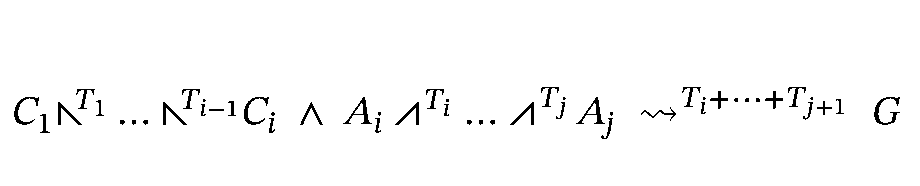
\includegraphics[scale=0.4]{pictures/schema-not-decorated.png}}
    \only<2->{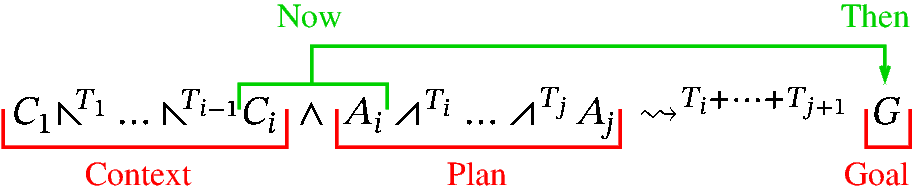
\includegraphics[scale=0.4]{pictures/schema-decorated.png}}
  \end{center}

  % <SPEECH>
  % Well, in a way everything is happening now, because, you remember I
  % said that this operator brings the past into the present, and that
  % one, and that one too, brings the future into the present, so
  % everything is from the viewpoint of the present.  But of course we
  % can't evaluate what is coming from the future, but everything else
  % we can.  So for instance if t is now, then we can evaluate

  \pause
  \pause

  {\large
    $$
    \begin{array}{ccc}
      \left[ C_1 \lbseqand{\!\! T_1} \dots \lbseqand{\!\! T_{i-1}} C_i
      \right](t) & = & \textit{True}\ |\ \textit{False}\\
      \pause & \mapsto & \mathcal{Dist}(Bool) \\
      \pause & \mapsto & \mathcal{Dist}(\mathcal{Dist}(Bool)) \\
    \end{array}
    $$
  }

  % And normally we should be able to evaluate to True or False, unless of
  % course the predicates are inherently uncertain, or we have forgotten
  % the past, etc, in which case it will be evaluated to a Bernouilli distribution,
  % possibly even a second order Bernouilli distribution.

\end{frame}

\end{document}
